\section{التحكم بالانزلاق (\LR{Sliding Mode Control - SMC})}
\label{sec:smc_control}

\subsection*{1. مبدأ الخوارزمية}
تُصنف خوارزمية التحكم بالانزلاق (\LR{SMC}) كواحدة من أقوى استراتيجيات التحكم اللاخطي المتين (\LR{Robust Control}). تعتمد الفكرة الأساسية على إجبار مسار النظام الديناميكي للوصول إلى سطح رياضي مصمم مسبقاً يُدعى "سطح الانزلاق" (\LR{Sliding Surface})، ثم إبقائه مقيداً على هذا السطح. يوفر هذا الأسلوب مناعة عالية جداً ضد التغيرات المعلمية (مثل تغير كتلة الحمل) والاضطرابات الخارجية.

\subsection*{2. الشكل العام لقانون التحكم}
يتكون قانون التحكم بالانزلاق من مركبين أساسيين:
\begin{equation}
u(t) = u_{eq}(t) + u_{sw}(t)
\end{equation}
حيث:
\begin{itemize}
    \item $u_{eq}$: قانون التحكم المكافئ (\LR{Equivalent Control})، وظيفته إبقاء النظام على السطح بافتراض عدم وجود اضطرابات (يعتمد على النموذج الاسمي).
    \item $u_{sw}$: قانون التبديل (\LR{Switching Control})، وظيفته التغلب على الشكوك ودفع النظام نحو السطح في حال انحرافه عنه.
\end{itemize}

\subsection*{3. تهيئة النموذج وتعريف الأخطاء}
باستخدام نفس تعريفات الخطأ الموضعي $e = q_{ref} - q$ وخطأ السرعة $\dot{e} = \dot{q}_{ref} - \dot{q}$، يتم تعريف شعاع سطح الانزلاق $S$ بأبعاد $3 \times 1$ لمفاصل الروبوت بالمعادلة:
\begin{equation}
S = \dot{e} + \Lambda e
\end{equation}
حيث $\Lambda$ مصفوفة قطرية موجبة تماماً تحدد ميل سطح الانزلاق وسرعة تقارب الخطأ نحو الصفر. 
بأخذ المشتق الزمني لسطح الانزلاق نحصل على:
\begin{equation}
\dot{S} = \ddot{e} + \Lambda \dot{e} = \ddot{q}_{ref} - \ddot{q} + \Lambda \dot{e}
\end{equation}

\subsection*{4. تطبيق الخوارزمية على النموذج}
بالاعتماد على النموذج الديناميكي الشامل للروبوت المستنتج في الفصل السابق: $\ddot{q} = \bar{M}^{-1} [A u - R \dot{q} - D]$، نقوم بتعويض $\ddot{q}$ في معادلة $\dot{S}$:
\begin{equation}
\dot{S} = \ddot{q}_{ref} - \bar{M}^{-1} [A u - R \dot{q} - D] + \Lambda \dot{e}
\end{equation}
لإيجاد التحكم المكافئ $u_{eq}$، نضع $\dot{S} = 0$، فنحصل على:
\begin{equation}
u_{eq} = A^{-1} \left[ \bar{M} (\ddot{q}_{ref} + \Lambda \dot{e}) + R \dot{q} + D \right]
\end{equation}
لضمان شرط الوصول لسطح الانزلاق (\LR{Reachability Condition}) في ظل وجود تغير في الكتلة، نضيف حد التبديل باختيار $u_{sw} = A^{-1} \bar{M} K \text{sgn}(S)$، حيث $K$ مصفوفة أرباح التبديل القطرية. ليصبح قانون التحكم النهائي المطبق على المحركات:
\begin{equation}
u_{SMC} = A^{-1} \left[ \bar{M} (\ddot{q}_{ref} + \Lambda \dot{e}) + R \dot{q} + D + K \text{sgn}(S) \right]
\end{equation}

\subsection{5. استجابة النظام عند قيم مختلفة للحمل ($m_L$)}
تم اختبار خوارزمية (\LR{SMC}) على نفس المسارات المرجعية السابقة ($\theta_{1ref} = \theta_{2ref} = 90^\circ$ و $d_{3ref} = 0.2 \text{ m}$). توضح الأشكال التالية متانة المتحكم عند تغير الحمل:


 \begin{figure}[H]
     \centering
     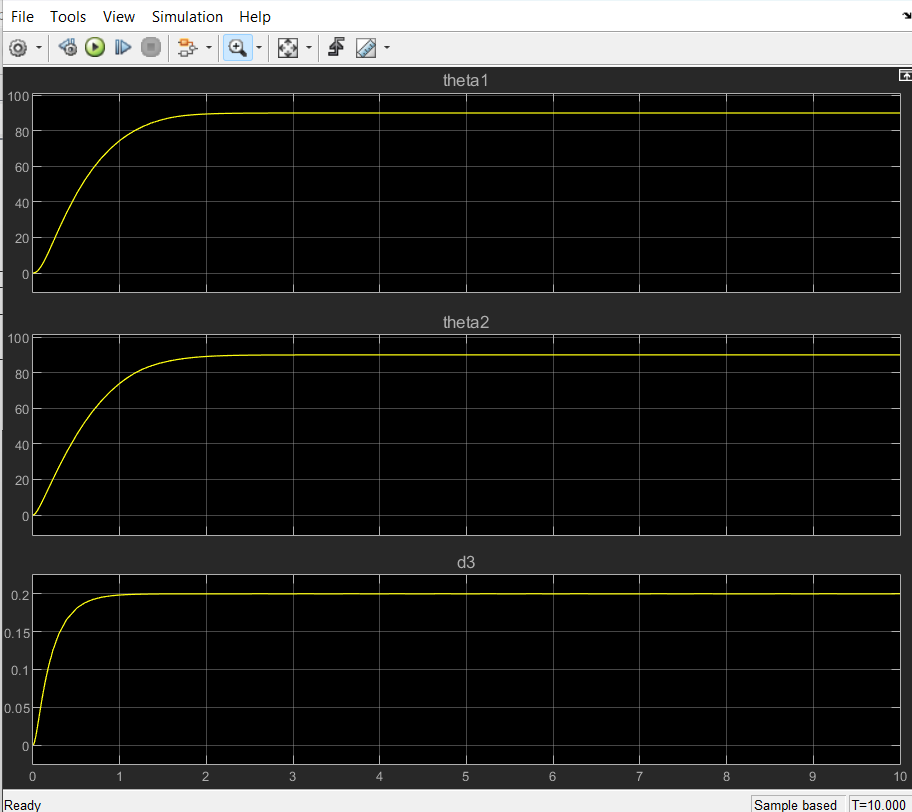
\includegraphics[width=0.8\textwidth]{resources/images/SMC_res_m0.png}
     \caption{\centering{استجابة متحكم \LR{SMC} بدون حمل ($m_L = 0 \text{ kg}$)}}
     \label{fig:smc_m0}
 \end{figure}

 \begin{figure}[H]
     \centering
     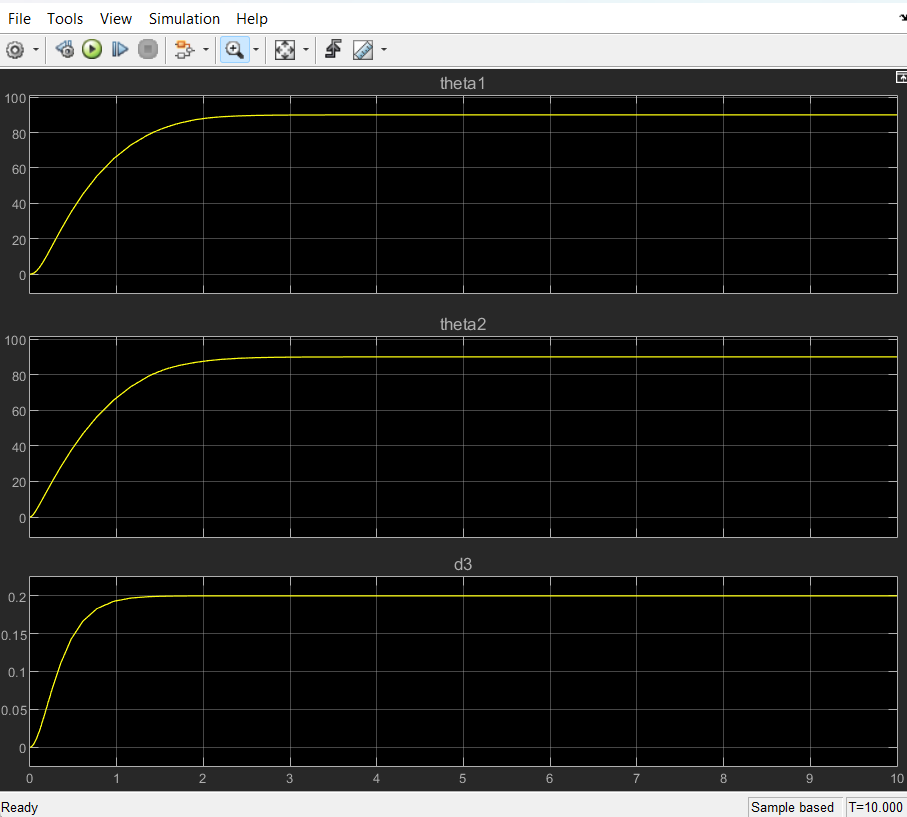
\includegraphics[width=0.8\textwidth]{resources/images/SMC_res_m10.png}
     \caption{\centering{استجابة متحكم \LR{SMC} عند إضافة حمل ($m_L = 10 \text{ kg}$)}}
     \label{fig:smc_m10}
 \end{figure}

على عكس الانهيار الذي حدث في خوارزمية (\LR{PID})، يُلاحظ من المنحنيات أن متحكم (\LR{SMC}) حافظ على دقة تتبع عالية للمسار المرجعي واستقرار ممتاز في المفصل الانسحابي حتى عند إضافة الحمل الأقصى ($10 kg$)، حيث استغرق النظام زمناً يقارب ($1 sec$) ليصل إلى حالة الاستقرار التام. يعود هذا الأداء المتين إلى تأثير حد التبديل اللاخطي الذي يجبر النظام على البقاء ضمن سطح الانزلاق المنيع ضد الاضطرابات الخارجية وتغيرات القصور الذاتي.